\documentclass[aspectratio=169,professionalfonts]{beamer}

\usetheme{Boadilla}
\usecolortheme{seahorse}

\usepackage[T1]{fontenc}
\usepackage{amsmath}
\usepackage{booktabs}
\usepackage{listings}
\usepackage{minted}
\usepackage{tikz}
\usetikzlibrary{arrows.meta,positioning,shapes.geometric}

\definecolor{mmblue}{RGB}{20,82,143}
\definecolor{mmteal}{RGB}{14,116,144}
\definecolor{mmgreen}{RGB}{22,101,52}
\definecolor{mmgray}{RGB}{75,85,99}
\definecolor{mmlight}{RGB}{243,244,246}
\definecolor{mmsignal}{RGB}{126,34,206}

\setbeamertemplate{navigation symbols}{}
\setbeamertemplate{footline}[frame number]
\setbeamercolor{title}{fg=mmblue}
\setbeamercolor{frametitle}{fg=mmblue}
\setbeamercolor{structure}{fg=mmblue}

\lstset{
  basicstyle=\ttfamily\small,
  columns=fullflexible,
  keepspaces=true,
  showstringspaces=false,
  frame=single,
  backgroundcolor=\color{mmlight}
}

\setminted{
  fontsize=\small,
  breaklines,
  bgcolor=mmlight
}

\title{How to Design a High Performance GEMM Kernel (on B200)?}
\subtitle{A practical optimization path from first principles to MMComposer}
\author{}
\date{\today}

\newcommand{\code}[1]{\texttt{#1}}

\begin{document}

\begin{frame}
  \titlepage
\end{frame}

\begin{frame}{Talk Outline}
  \begin{itemize}
    \item GEMM breakdown.
    \item The core idea: a GEMM kernel is an orchestration problem.
    \item From diagram to code: how the synchronization actually looks.
    \item MMComposer: how to use it to generate GEMM kernels.
  \end{itemize}
\end{frame}

\section{Background}


\begin{frame}{GEMM Breakdown}
  A GEMM kernel has two major phases: \textbf{compute} and \textbf{epilogue}.

  \vspace{0.35cm}
  \begin{columns}[T,onlytextwidth]
    \column{0.48\textwidth}
    \textbf{Compute}
    \begin{itemize}
      \item Fetch A/B tiles.
      \item Stage tiles in shared memory.
      \item Issue MMA instructions.
      \item Accumulate results in TMEM.
    \end{itemize}

    \column{0.48\textwidth}
    \textbf{Epilogue}
    \begin{itemize}
      \item Load TMEM into registers.
      \item Apply optional operations such as ReLU or SwiGLU.
      \item Pack registers into shared memory.
      \item Store the final result to HBM.
    \end{itemize}
  \end{columns}
\end{frame}

\section{Orchestration}

\begin{frame}{The Core Idea: Orchestration}
  If there is one idea to take away from this talk, it is this:

  \vspace{0.35cm}
  \begin{center}
    \textbf{A high-performance GEMM kernel is an orchestration problem.}
  \end{center}

  \vspace{0.35cm}
  The kernel is a dataflow schedule over hardware units, warp roles, and
  on-chip containers. Performance depends on keeping values flowing while
  reusing scarce containers at the right time.
\end{frame}

\begin{frame}{Operations and Containers}
  Think of each operation as:

  \vspace{0.25cm}
  \begin{center}
    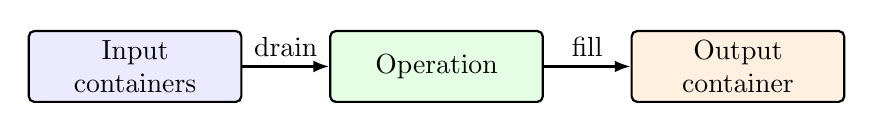
\begin{tikzpicture}[
        box/.style={draw, thick, rounded corners=2pt, minimum width=2.7cm, minimum height=0.9cm, align=center},
        arrow/.style={-{Latex[length=2mm]}, thick}
      ]
      \node[box, fill=blue!8] (in) {Input\\containers};
      \node[box, fill=green!10, right=1.1cm of in] (op) {Operation};
      \node[box, fill=orange!12, right=1.1cm of op] (out) {Output\\container};
      \draw[arrow] (in) -- node[above]{drain} (op);
      \draw[arrow] (op) -- node[above]{fill} (out);
    \end{tikzpicture}
  \end{center}

  \vspace{0.25cm}
  \begin{itemize}
    \item An operation consumes one or more input values from containers.
    \item It produces one output value into another container.
    \item It can start only when its input values are ready and its output container is free.
    \item Once an input has been fully drained, its container is free to reuse.
    \item Once the output has been fully computed, it is ready to be consumed.
  \end{itemize}
\end{frame}

\begin{frame}{When Can an Operation Start?}
  An operation is schedulable only when both conditions are true:

  \vspace{0.25cm}
  \begin{enumerate}
    \item \textbf{Input value-ready}: every input value it needs has been produced.
    \item \textbf{Output resource-free}: the container for its output is available.
  \end{enumerate}

  \vspace{0.3cm}
  In other words, the operation is blocked if either the data is not ready
  or the destination container is still occupied.

  \vspace{0.25cm}
  This is the basic rule behind SMEM ring-buffer reuse, TMEM reuse, and TMA
  store-buffer pipelining.
\end{frame}

\begin{frame}{Two Signals}
  In this model, synchronization has two meanings:

  \begin{enumerate}
    \item \textbf{Data-ready}: a container is full; data is ready to be consumed.
    \item \textbf{Resource-free}: a container is empty; it can be reused.
  \end{enumerate}

  \vspace{0.3cm}
  A producer is waiting for a free output container. A consumer is waiting for
  a ready input value. Good GEMM scheduling is mostly about making those two
  waits overlap with useful work.

  \vspace{0.15cm}
  For TMEM, value readiness is gated by a completion condition: the
  \textbf{TMEM data ready} signal is sent only after the final MMA finishes.

  \vspace{0.25cm}
  \begin{center}
    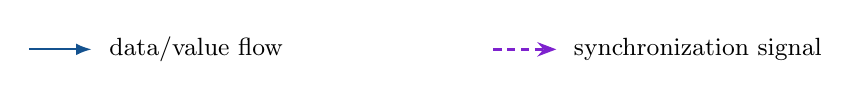
\begin{tikzpicture}[
        flow/.style={-{Latex[length=2mm]}, thick},
        signal/.style={-{Stealth[length=2.4mm]}, very thick, densely dashed}
      ]
      \draw[flow, draw=mmblue] (-4.6,0) -- (-3.8,0);
      \node[right] at (-3.7,0) {\small data/value flow};
      \draw[signal, draw=mmsignal] (1.3,0) -- (2.1,0);
      \node[right] at (2.2,0) {\small synchronization signal};
    \end{tikzpicture}
  \end{center}
\end{frame}

\begin{frame}{Dataflow Alone Is Not Enough}
  The high-level dataflow is simple:

  \vspace{0.3cm}
  \begin{center}
    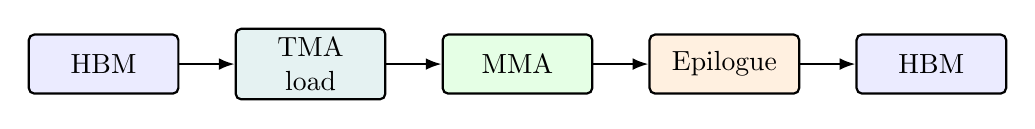
\begin{tikzpicture}[
        node/.style={draw, thick, rounded corners=2pt, minimum width=1.9cm, minimum height=0.75cm, align=center},
        arrow/.style={-{Latex[length=2mm]}, thick}
      ]
      \node[node, fill=blue!8] (hbm0) {HBM};
      \node[node, fill=teal!10, right=0.7cm of hbm0] (tma) {TMA\\load};
      \node[node, fill=green!10, right=0.7cm of tma] (mma) {MMA};
      \node[node, fill=orange!12, right=0.7cm of mma] (epi) {Epilogue};
      \node[node, fill=blue!8, right=0.7cm of epi] (hbm1) {HBM};
      \draw[arrow] (hbm0) -- (tma);
      \draw[arrow] (tma) -- (mma);
      \draw[arrow] (mma) -- (epi);
      \draw[arrow] (epi) -- (hbm1);
    \end{tikzpicture}
  \end{center}

  \vspace{0.3cm}
  But this diagram hides the most important scheduling question:

  \vspace{0.15cm}
  \begin{center}
    \textbf{Where is each value stored while it waits for the next operation?}
  \end{center}
\end{frame}

\begin{frame}{Add the Containers}
  For the synchronization model used in this talk, we group the kernel into
  three producer/consumer operations:

  \begin{table}
    \centering
    \scriptsize
    \begin{tabular}{lll}
      \toprule
      Operation & Input container & Output container \\
      \midrule
      TMA warps & HBM A/B tiles & SMEM compute ring buffer \\
      MMA warps & SMEM compute ring buffer & TMEM accumulator \\
      Epilogue warps & TMEM accumulator & registers \\
      \bottomrule
    \end{tabular}
  \end{table}

  \vspace{0.2cm}
  This is the abstraction used in the next graph. The epilogue's internal
  pack and TMA-store staging are real, but they are not the main
  warp-to-warp synchronization edges shown here.
\end{frame}


\begin{frame}{Main Synchronization Pattern: Graph View}
  \begin{center}
    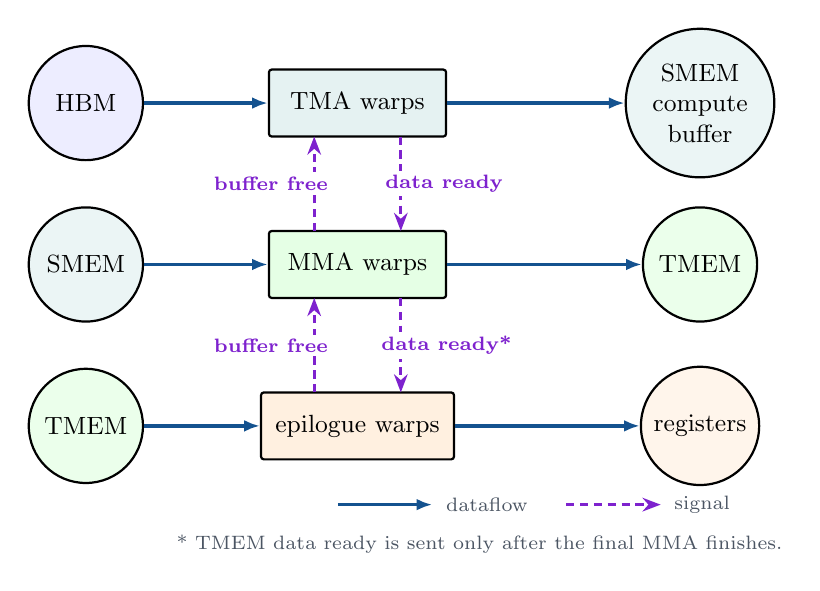
\begin{tikzpicture}[
        container/.style={circle, draw, thick, minimum size=1.45cm, align=center, font=\small},
        op/.style={draw, thick, rounded corners=1pt, minimum width=2.25cm, minimum height=0.85cm, align=center, font=\small},
        flow/.style={-{Latex[length=2mm]}, very thick, draw=mmblue},
        signal/.style={-{Stealth[length=2.3mm]}, very thick, densely dashed},
        siglabel/.style={font=\scriptsize\bfseries, align=center, inner sep=1.5pt, fill=white}
      ]
      \node[container, fill=blue!7] (hbm1) at (-5.0,2.05) {HBM};
      \node[op, fill=teal!10] (tma) at (-1.55,2.05) {TMA warps};
      \node[container, fill=teal!8, minimum size=1.75cm] (smem1) at (2.8,2.05) {SMEM\\compute\\buffer};

      \node[container, fill=teal!8] (smem2) at (-5.0,0) {SMEM};
      \node[op, fill=green!10] (mma) at (-1.55,0) {MMA warps};
      \node[container, fill=green!8] (tmem2) at (2.8,0) {TMEM};

      \node[container, fill=green!8] (tmem3) at (-5.0,-2.05) {TMEM};
      \node[op, fill=orange!12, minimum width=2.45cm] (epi) at (-1.55,-2.05) {epilogue warps};
      \node[container, fill=orange!8] (regs) at (2.8,-2.05) {registers};

      \draw[flow] (hbm1) -- (tma);
      \draw[flow] (tma) -- (smem1);
      \draw[flow] (smem2) -- (mma);
      \draw[flow] (mma) -- (tmem2);
      \draw[flow] (tmem3) -- (epi);
      \draw[flow] (epi) -- (regs);

      \draw[signal, draw=mmsignal] (-1.00,1.625) -- (-1.00,0.425);
      \node[siglabel, text=mmsignal] at (-0.45,1.03) {data ready};

      \draw[signal, draw=mmsignal] (-2.10,0.425) -- (-2.10,1.625);
      \node[siglabel, text=mmsignal] at (-2.65,1.03) {buffer free};

      \draw[signal, draw=mmsignal] (-1.00,-0.425) -- (-1.00,-1.625);
      \node[siglabel, text=mmsignal] at (-0.42,-1.03) {data ready*};

      \draw[signal, draw=mmsignal] (-2.10,-1.625) -- (-2.10,-0.425);
      \node[siglabel, text=mmsignal] at (-2.65,-1.03) {buffer free};

      \draw[flow] (-1.8,-3.05) -- (-0.6,-3.05);
      \node[font=\scriptsize, text=mmgray, right] at (-0.55,-3.05) {dataflow};
      \draw[signal, draw=mmsignal] (1.1,-3.05) -- (2.3,-3.05);
      \node[font=\scriptsize, text=mmgray, right] at (2.35,-3.05) {signal};
      \node[font=\scriptsize, text=mmgray, align=center] at (0,-3.55)
        {* TMEM data ready is sent only after the final MMA finishes.};
    \end{tikzpicture}
  \end{center}
\end{frame}

\begin{frame}{TMA Warps: Fill SMEM, Signal Data Ready}
  \begin{center}
    \begin{tikzpicture}[
        container/.style={circle, draw=black!25, thick, minimum size=1.45cm, align=center, font=\small, fill=black!4, text=black!45},
        activecontainer/.style={circle, draw, thick, minimum size=1.45cm, align=center, font=\small},
        op/.style={draw=black!25, thick, rounded corners=1pt, minimum width=2.25cm, minimum height=0.85cm, align=center, font=\small, fill=black!4, text=black!45},
        activeop/.style={draw, thick, rounded corners=1pt, minimum width=2.25cm, minimum height=0.85cm, align=center, font=\small},
        flow/.style={-{Latex[length=2mm]}, very thick, draw=black!25},
        activeflow/.style={-{Latex[length=2mm]}, very thick, draw=mmblue},
        signal/.style={-{Stealth[length=2.3mm]}, very thick, densely dashed, draw=black!25},
        activesignal/.style={-{Stealth[length=2.3mm]}, very thick, densely dashed, draw=mmsignal},
        siglabel/.style={font=\scriptsize\bfseries, align=center, inner sep=1.5pt, fill=white},
        status/.style={font=\scriptsize, text=mmgray}
      ]
      \node[activecontainer, fill=blue!4] (hbm1) at (-5.0,2.05) {};
      \begin{scope}
        \clip (-5.0,2.05) circle (0.725cm);
        \only<1>{\fill[blue!25] (-5.725,1.325) rectangle (-4.275,2.775);}
        \only<2>{\fill[blue!25] (-5.725,1.325) rectangle (-4.275,2.05);}
      \end{scope}
      \node[activecontainer] at (hbm1) {};
      \node[font=\small] at (hbm1) {HBM};

      \node[activeop, fill=teal!10] (tma) at (-1.55,2.05) {TMA warps};

      \node[activecontainer, fill=teal!4, minimum size=1.75cm] (smem1) at (2.8,2.05) {};
      \begin{scope}
        \clip (2.8,2.05) circle (0.875cm);
        \only<2>{\fill[teal!28] (1.925,1.175) rectangle (3.675,2.05);}
        \only<3>{\fill[teal!28] (1.925,1.175) rectangle (3.675,2.925);}
      \end{scope}
      \node[activecontainer, minimum size=1.75cm] at (smem1) {};
      \node[font=\small, align=center] at (smem1) {SMEM\\compute\\buffer};

      \node[container] (smem2) at (-5.0,0) {SMEM};
      \node[op] (mma) at (-1.55,0) {MMA warps};
      \node[container] (tmem2) at (2.8,0) {TMEM};

      \node[container] (tmem3) at (-5.0,-2.05) {TMEM};
      \node[op, minimum width=2.45cm] (epi) at (-1.55,-2.05) {epilogue warps};
      \node[container] (regs) at (2.8,-2.05) {registers};

      \draw[activeflow] (hbm1) -- node[above, font=\scriptsize, text=mmblue] {drain} (tma);
      \draw[activeflow] (tma) -- node[above, font=\scriptsize, text=mmblue] {fill} (smem1);
      \draw[flow] (smem2) -- (mma);
      \draw[flow] (mma) -- (tmem2);
      \draw[flow] (tmem3) -- (epi);
      \draw[flow] (epi) -- (regs);

      \only<1-2>{\draw[signal] (-1.00,1.625) -- (-1.00,0.425);}
      \only<3>{
        \draw[activesignal] (-1.00,1.625) -- (-1.00,0.425);
        \node[siglabel, text=mmsignal] at (-0.45,1.03) {data ready};
      }
      \draw[signal] (-2.10,0.425) -- (-2.10,1.625);
      \draw[signal] (-1.00,-0.425) -- (-1.00,-1.625);
      \draw[signal] (-2.10,-1.625) -- (-2.10,-0.425);

      \node[status] at (-5.0,1.08) {
        \only<1>{full}
        \only<2>{half full}
        \only<3>{empty}
      };
      \node[status] at (2.8,0.93) {
        \only<1>{empty}
        \only<2>{half full}
        \only<3>{full}
      };
    \end{tikzpicture}
  \end{center}

  \vspace{-0.15cm}
  \only<1>{The TMA operation can start: the HBM tile is ready, and the SMEM
  compute slot is free.}
  \only<2>{The TMA warps drain the HBM tile while filling the SMEM compute
  slot.}
  \only<3>{Once the HBM tile is drained and the SMEM slot is full, the TMA
  warps send \textbf{compute data ready} to the MMA warps.}
\end{frame}

\begin{frame}{MMA Warps: Signal Buffer Free and Data Ready}
  \begin{center}
    \begin{tikzpicture}[
        container/.style={circle, draw=black!25, thick, minimum size=1.45cm, align=center, font=\small, fill=black!4, text=black!45},
        activecontainer/.style={circle, draw, thick, minimum size=1.45cm, align=center, font=\small},
        op/.style={draw=black!25, thick, rounded corners=1pt, minimum width=2.25cm, minimum height=0.85cm, align=center, font=\small, fill=black!4, text=black!45},
        activeop/.style={draw, thick, rounded corners=1pt, minimum width=2.25cm, minimum height=0.85cm, align=center, font=\small},
        flow/.style={-{Latex[length=2mm]}, very thick, draw=black!25},
        activeflow/.style={-{Latex[length=2mm]}, very thick, draw=mmblue},
        signal/.style={-{Stealth[length=2.3mm]}, very thick, densely dashed, draw=black!25},
        activesignal/.style={-{Stealth[length=2.3mm]}, very thick, densely dashed, draw=mmsignal},
        siglabel/.style={font=\scriptsize\bfseries, align=center, inner sep=1.5pt, fill=white},
        status/.style={font=\scriptsize, text=mmgray}
      ]
      \node[container] (hbm1) at (-5.0,2.05) {HBM};
      \node[op] (tma) at (-1.55,2.05) {TMA warps};
      \node[container, minimum size=1.75cm] (smem1) at (2.8,2.05) {SMEM\\compute\\buffer};

      \node[activecontainer, fill=teal!4] (smem2) at (-5.0,0) {};
      \begin{scope}
        \clip (-5.0,0) circle (0.725cm);
        \only<1>{\fill[teal!28] (-5.725,-0.725) rectangle (-4.275,0.725);}
        \only<2>{\fill[teal!28] (-5.725,-0.725) rectangle (-4.275,0);}
      \end{scope}
      \node[activecontainer] at (smem2) {};
      \node[font=\small] at (smem2) {SMEM};

      \node[activeop, fill=green!10] (mma) at (-1.55,0) {MMA warps};

      \node[activecontainer, fill=green!4] (tmem2) at (2.8,0) {};
      \begin{scope}
        \clip (2.8,0) circle (0.725cm);
        \only<2>{\fill[green!28] (2.075,-0.725) rectangle (3.525,0);}
        \only<3-4>{\fill[green!28] (2.075,-0.725) rectangle (3.525,0.725);}
      \end{scope}
      \node[activecontainer] at (tmem2) {};
      \node[font=\small] at (tmem2) {TMEM};

      \node[container] (tmem3) at (-5.0,-2.05) {TMEM};
      \node[op, minimum width=2.45cm] (epi) at (-1.55,-2.05) {epilogue warps};
      \node[container] (regs) at (2.8,-2.05) {registers};

      \draw[flow] (hbm1) -- (tma);
      \draw[flow] (tma) -- (smem1);
      \draw[activeflow] (smem2) -- node[above, font=\scriptsize, text=mmblue] {drain} (mma);
      \draw[activeflow] (mma) -- node[above, font=\scriptsize, text=mmblue] {fill} (tmem2);
      \draw[flow] (tmem3) -- (epi);
      \draw[flow] (epi) -- (regs);

      \draw[signal] (-1.00,1.625) -- (-1.00,0.425);
      \only<1-2,4>{\draw[signal] (-2.10,0.425) -- (-2.10,1.625);}
      \only<3>{
        \draw[activesignal] (-2.10,0.425) -- (-2.10,1.625);
        \node[siglabel, text=mmsignal] at (-2.65,1.03) {buffer free};
      }
      \only<1-3>{\draw[signal] (-1.00,-0.425) -- (-1.00,-1.625);}
      \only<4>{
        \draw[activesignal] (-1.00,-0.425) -- (-1.00,-1.625);
        \node[siglabel, text=mmsignal] at (-0.42,-1.03) {data ready*};
      }
      \draw[signal] (-2.10,-1.625) -- (-2.10,-0.425);

      \node[status] at (-5.0,-0.98) {
        \only<1>{full}
        \only<2>{half full}
        \only<3-4>{empty}
      };
      \node[status] at (2.8,-0.98) {
        \only<1>{empty}
        \only<2>{half full}
        \only<3-4>{full}
      };
    \end{tikzpicture}
  \end{center}

  \vspace{-0.15cm}
  \only<1>{The MMA operation can start: compute data is ready in SMEM, and the
  TMEM accumulator buffer is free.}
  \only<2>{The MMA warps drain the SMEM compute buffer while filling TMEM.}
  \only<3>{Once the SMEM input is drained, the MMA warps send
  \textbf{compute buffer free} back to TMA.}
  \only<4>{After the final MMA for this output tile, the MMA warps send
  \textbf{TMEM data ready} to the epilogue warps.\\[-0.05cm]
  \footnotesize * data ready is sent only after the final MMA finishes.}
\end{frame}

\begin{frame}{Epilogue Warps: Drain TMEM, Signal Buffer Free}
  \begin{center}
    \begin{tikzpicture}[
        container/.style={circle, draw=black!25, thick, minimum size=1.45cm, align=center, font=\small, fill=black!4, text=black!45},
        activecontainer/.style={circle, draw, thick, minimum size=1.45cm, align=center, font=\small},
        op/.style={draw=black!25, thick, rounded corners=1pt, minimum width=2.25cm, minimum height=0.85cm, align=center, font=\small, fill=black!4, text=black!45},
        activeop/.style={draw, thick, rounded corners=1pt, minimum width=2.45cm, minimum height=0.85cm, align=center, font=\small},
        flow/.style={-{Latex[length=2mm]}, very thick, draw=black!25},
        activeflow/.style={-{Latex[length=2mm]}, very thick, draw=mmblue},
        signal/.style={-{Stealth[length=2.3mm]}, very thick, densely dashed, draw=black!25},
        activesignal/.style={-{Stealth[length=2.3mm]}, very thick, densely dashed, draw=mmsignal},
        siglabel/.style={font=\scriptsize\bfseries, align=center, inner sep=1.5pt, fill=white},
        status/.style={font=\scriptsize, text=mmgray}
      ]
      \node[container] (hbm1) at (-5.0,2.05) {HBM};
      \node[op] (tma) at (-1.55,2.05) {TMA warps};
      \node[container, minimum size=1.75cm] (smem1) at (2.8,2.05) {SMEM\\compute\\buffer};

      \node[container] (smem2) at (-5.0,0) {SMEM};
      \node[op] (mma) at (-1.55,0) {MMA warps};
      \node[container] (tmem2) at (2.8,0) {TMEM};

      \node[activecontainer, fill=green!4] (tmem3) at (-5.0,-2.05) {};
      \begin{scope}
        \clip (-5.0,-2.05) circle (0.725cm);
        \only<1>{\fill[green!28] (-5.725,-2.775) rectangle (-4.275,-1.325);}
        \only<2>{\fill[green!28] (-5.725,-2.775) rectangle (-4.275,-2.05);}
      \end{scope}
      \node[activecontainer] at (tmem3) {};
      \node[font=\small] at (tmem3) {TMEM};

      \node[activeop, fill=orange!12] (epi) at (-1.55,-2.05) {epilogue warps};

      \node[activecontainer, fill=orange!4] (regs) at (2.8,-2.05) {};
      \begin{scope}
        \clip (2.8,-2.05) circle (0.725cm);
        \only<2>{\fill[orange!28] (2.075,-2.775) rectangle (3.525,-2.05);}
        \only<3>{\fill[orange!28] (2.075,-2.775) rectangle (3.525,-1.325);}
      \end{scope}
      \node[activecontainer] at (regs) {};
      \node[font=\small] at (regs) {registers};

      \draw[flow] (hbm1) -- (tma);
      \draw[flow] (tma) -- (smem1);
      \draw[flow] (smem2) -- (mma);
      \draw[flow] (mma) -- (tmem2);
      \draw[activeflow] (tmem3) -- node[above, font=\scriptsize, text=mmblue] {drain} (epi);
      \draw[activeflow] (epi) -- node[above, font=\scriptsize, text=mmblue] {fill} (regs);

      \draw[signal] (-1.00,1.625) -- (-1.00,0.425);
      \draw[signal] (-2.10,0.425) -- (-2.10,1.625);
      \draw[signal] (-1.00,-0.425) -- (-1.00,-1.625);
      \only<1-2>{\draw[signal] (-2.10,-1.625) -- (-2.10,-0.425);}
      \only<3>{
        \draw[activesignal] (-2.10,-1.625) -- (-2.10,-0.425);
        \node[siglabel, text=mmsignal] at (-2.65,-1.03) {buffer free};
      }

      \node[status] at (-5.0,-3.03) {
        \only<1>{full}
        \only<2>{half full}
        \only<3>{empty}
      };
      \node[status] at (2.8,-3.03) {
        \only<1>{empty}
        \only<2>{half full}
        \only<3>{full}
      };
    \end{tikzpicture}
  \end{center}

  \vspace{-0.15cm}
  \only<1>{The epilogue can start: TMEM data is ready, and the register
  destination is available.}
  \only<2>{The epilogue warps drain TMEM while filling registers.}
  \only<3>{Once TMEM is drained, the epilogue warps send
  \textbf{TMEM buffer free} back to the MMA warps.}
\end{frame}

\begin{frame}{Using Multiple Buffers}
  \small
  The single-container graph is the dependency for one slot. Real kernels
  replicate the same ready/free protocol across multiple slots.

  \vspace{0.05cm}
  \begin{center}
    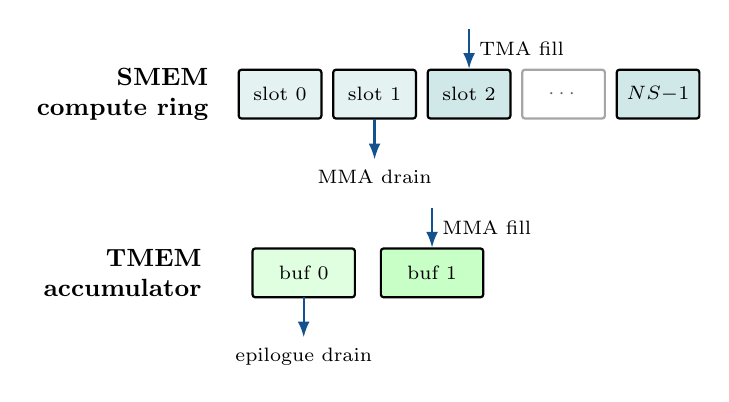
\begin{tikzpicture}[
        slot/.style={draw, thick, rounded corners=1pt, minimum width=1.05cm, minimum height=0.62cm, align=center, font=\scriptsize},
        label/.style={font=\small\bfseries, align=right},
        note/.style={font=\scriptsize, text=mmgray, align=left, anchor=west},
        flow/.style={-{Latex[length=2mm]}, thick, draw=mmblue},
        signal/.style={-{Stealth[length=2mm]}, thick, densely dashed, draw=mmsignal}
      ]
      \node[label] at (-4.75,0.92) {SMEM\\compute ring};
      \node[slot, fill=teal!10] (s0) at (-2.75,0.92) {slot 0};
      \node[slot, fill=teal!10] (s1) at (-1.55,0.92) {slot 1};
      \node[slot, fill=teal!18] (s2) at (-0.35,0.92) {slot 2};
      \node[slot, draw=black!35, text=black!60] (sd) at (0.85,0.92) {$\cdots$};
      \node[slot, fill=teal!18] (sn) at (2.05,0.92) {$NS{-}1$};
      \draw[flow] (-1.55,0.60) -- (-1.55,0.09)
        node[below, font=\scriptsize] {MMA drain};
      \draw[flow] (-0.35,1.75) -- (-0.35,1.24)
        node[midway, right, font=\scriptsize] {TMA fill};

      \node[label] at (-4.75,-1.35) {TMEM\\accumulator};
      \node[slot, fill=green!12, minimum width=1.30cm] (t0) at (-2.45,-1.35) {buf 0};
      \node[slot, fill=green!22, minimum width=1.30cm] (t1) at (-0.82,-1.35) {buf 1};
      \draw[flow] (-2.45,-1.66) -- (-2.45,-2.17)
        node[below, font=\scriptsize] {epilogue drain};
      \draw[flow] (-0.82,-0.52) -- (-0.82,-1.03)
        node[midway, right, font=\scriptsize] {MMA fill};
    \end{tikzpicture}
  \end{center}

  \vspace{-0.18cm}
  \begin{table}
    \centering
    \scriptsize
    \begin{tabular}{lll}
      \toprule
      Container & Buffering & Effect \\
      \midrule
      SMEM compute ring & $NS$ slots &
        MMA consumes one slot while TMA fills the next. \\
      TMEM accumulator & 2 buffers &
        Epilogue drains the previous output while MMA produces the next. \\
      \bottomrule
    \end{tabular}
  \end{table}
\end{frame}

\begin{frame}{Deriving the Warp Roles}
  \begin{table}
    \centering
    \small
    \begin{tabular}{llll}
      \toprule
      Worker & Drains & Fills & Key signal \\
      \midrule
      TMA warp & HBM tile & SMEM compute ring & compute data ready \\
      MMA warp & SMEM compute ring & TMEM &
        \begin{tabular}[c]{@{}l@{}}compute buffer free\\TMEM data ready\end{tabular} \\
      Epilogue warp & TMEM & registers & TMEM buffer free \\
      TMA store path & SMEM store ring & HBM output & store slot free \\
      \bottomrule
    \end{tabular}
  \end{table}

  \vspace{0.2cm}
  The same rule repeats: drain an input container, fill an output container,
  then signal readiness, completion, or resource reuse.
\end{frame}

\section{2-CTA MMA}

\begin{frame}{One Optimization the Model Does Not Imply: 2-CTA MMA}
  The orchestration model already covers warp specialization, pipelining,
  SMEM/TMEM reuse, and epilogue overlap. One major B200 optimization is
  \emph{not} implied by it:

  \vspace{0.3cm}
  \begin{center}
    \textbf{2-CTA MMA}: two CTAs in a cluster cooperate on one MMA.
  \end{center}

  \vspace{0.3cm}
  \begin{itemize}
    \item Form a cluster of 2 CTAs (\code{\_\_cluster\_dims\_\_(2,1,1)}).
    \item Issue a single \code{tcgen05.mma.cta\_group::2} across the pair.
    \item The pair produces a $2\,BM \times BN$ output tile per MMA.
  \end{itemize}
\end{frame}

\begin{frame}{2-CTA MMA: Geometry}
  \begin{columns}[T,onlytextwidth]
    \column{0.52\textwidth}
    \begin{itemize}
      \item Each CTA owns \textbf{half of B}: $BN_{\text{local}} = BN/2$.
      \item Both CTAs load the \textbf{full A} rows for their $BM$.
      \item Per-CTA SMEM per slot drops from 48\,KB to \textbf{32\,KB} (at $BN{=}256$).
      \item TMA loads use \code{.cta\_group::2}; the \code{tcgen05.commit}
        multicasts the completion signal to both CTAs.
    \end{itemize}

    \column{0.46\textwidth}
    \begin{center}
      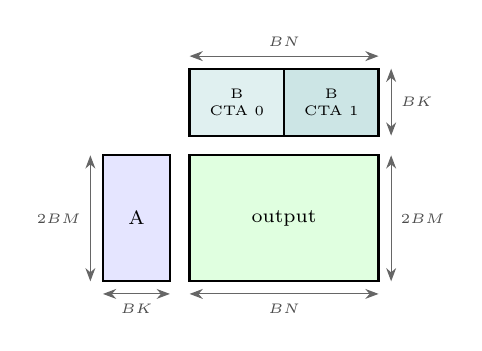
\begin{tikzpicture}[
          lab/.style={align=center, font=\scriptsize},
          bhlab/.style={align=center, font=\tiny},
          dim/.style={Stealth-Stealth, thin, black!60},
          dimlab/.style={font=\tiny, text=black!70}
        ]
        % Fixed-coordinate geometry:
        % A width = B height = BK, and B total width = output width = BN.
        \draw[thick, fill=blue!10]  (0,0) rectangle (0.85,1.60);
        \draw[thick, fill=green!12] (1.10,0) rectangle (3.50,1.60);
        \draw[thick, fill=teal!12]  (1.10,1.85) rectangle (2.30,2.70);
        \draw[thick, fill=teal!20]  (2.30,1.85) rectangle (3.50,2.70);

        \node[lab] at (0.425,0.80) {A};
        \node[lab] at (2.30,0.80) {output};
        \node[bhlab] at (1.70,2.275) {B\\CTA 0};
        \node[bhlab] at (2.90,2.275) {B\\CTA 1};

        \draw[dim] (0,-0.16) -- (0.85,-0.16)
            node[midway, below, dimlab] {$BK$};
        \draw[dim] (-0.16,0) -- (-0.16,1.60)
            node[midway, left, dimlab] {$2BM$};
        \draw[dim] (1.10,-0.16) -- (3.50,-0.16)
            node[midway, below, dimlab] {$BN$};
        \draw[dim] (3.66,0) -- (3.66,1.60)
            node[midway, right, dimlab] {$2BM$};
        \draw[dim] (1.10,2.86) -- (3.50,2.86)
            node[midway, above, dimlab] {$BN$};
        \draw[dim] (3.66,1.85) -- (3.66,2.70)
            node[midway, right, dimlab] {$BK$};
      \end{tikzpicture}
    \end{center}
  \end{columns}
\end{frame}

\begin{frame}[fragile]{2-CTA MMA: In the Instructions}
  The cluster cooperation shows up directly in the PTX:
  \begin{lstlisting}[language=C]
// TMA load into clustered SMEM (both CTAs' arrivals counted):
cp.async.bulk.tensor.2d.shared::cluster.global
    .mbarrier::complete_tx::bytes.cta_group::2  [smem], [tmap,{x,y}], [mbar];

// One MMA issued across the CTA pair:
tcgen05.mma.cta_group::2.kind::f16  ... ;

// Completion multicast to both CTAs in the cluster:
tcgen05.commit.cta_group::2.mbarrier::arrive::one
    .shared::cluster.multicast::cluster.b64  [smem_compute_free_mbar], cta_mask;
  \end{lstlisting}
  \vspace{-0.2cm}
  \footnotesize Source: \code{webui/kernels/tier3\_cluster\_swizzle/kernel.cu}.
\end{frame}

\section{Tile Sizes and Shared Memory}

\begin{frame}{Framework Choice: Disjoint SMEM}
  There are several valid ways to share on-chip storage between compute and
  epilogue. In this talk, we will use one common framework:

  \begin{itemize}
    \item Compute uses a dedicated SMEM ring buffer for A/B tiles.
    \item The epilogue is \textbf{always a pipelined TMA store}: it packs results
      into a separate SMEM store ring buffer and lets TMA push tiles to HBM.
    \item The number of TMA store pipeline stages is a tunable parameter.
  \end{itemize}

  \vspace{0.2cm}
  This is not the only possible design, but it is a clean default that works
  well across many shapes. Its consequence: shared memory splits into
  \textbf{two} rings, and 2-CTA tile sizes set how big each one is.
\end{frame}

\begin{frame}{Partitioning Shared Memory}
  \begin{center}
    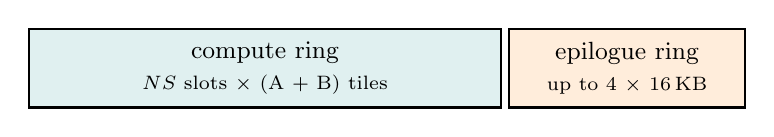
\begin{tikzpicture}[
        seg/.style={draw, thick, minimum height=1.0cm, align=center, font=\small}
      ]
      \node[seg, fill=teal!12, minimum width=6.0cm] (comp) at (0,0)
        {compute ring\\ \scriptsize $NS$ slots $\times$ (A + B) tiles};
      \node[seg, fill=orange!14, minimum width=3.0cm, right=2pt of comp] (epi)
        {epilogue ring\\ \scriptsize up to 4 $\times$ 16\,KB};
    \end{tikzpicture}
  \end{center}

  \vspace{0.1cm}
  \begin{itemize}
    \item \textbf{Compute ring}: $NS$ pipeline slots, each holding one A tile and
      one B tile for the MMA stage.
    \item \textbf{Epilogue ring}: the TMA store buffers. MMComposer exposes up to
      \textbf{4} store buffers, each \textbf{16\,KB}.
    \item Both rings share one per-SM SMEM budget, so larger tiles or deeper
      pipelines on one side leave less room for the other.
  \end{itemize}
\end{frame}

\begin{frame}{Tile Sizes and the SMEM Budget}
  Per compute slot (2-CTA, each CTA owns half of B):
  \[
    \text{slot} = \underbrace{BM\cdot BK\cdot 2}_{\text{A tile}}
                + \underbrace{\tfrac{BN}{2}\cdot BK\cdot 2}_{\text{B tile (local)}}
  \]

  \begin{table}
    \centering\small
    \begin{tabular}{lrrr}
      \toprule
      Config (2-CTA, $BK{=}64$) & A tile & B tile & slot \\
      \midrule
      $BM{=}128,\ BN{=}256$ & 16\,KB & 16\,KB & 32\,KB \\
      $BM{=}128,\ BN{=}512$ & 16\,KB & 32\,KB & 48\,KB \\
      \bottomrule
    \end{tabular}
  \end{table}

  \vspace{0.15cm}
  Budget constraint (per SM, B200 $\approx$ 228\,KB):
  \[
    \underbrace{NS \times \text{slot}}_{\text{compute ring}}
    \;+\;
    \underbrace{E \times 16\,\text{KB}}_{\text{epilogue ring},\ E\le 4}
    \;\le\; S_{\text{SMEM}}
  \]

  \footnotesize Example: $BN{=}256$, $NS{=}5 \Rightarrow 160$\,KB compute ring;
  with $E{=}2$ store buffers, $+32$\,KB $= 192$\,KB total.
  % TODO(tong): confirm the exact per-SM SMEM cap used (228 KB?).
\end{frame}

\section{From Diagram to Code}

\begin{frame}{From Diagram to Code}
  We now connect the container diagram to the real kernel. Each warp role maps
  to one loop that \emph{waits}, \emph{works}, then \emph{signals}:

  \vspace{0.3cm}
  \begin{table}
    \centering\scriptsize
    \begin{tabular}{llll}
      \toprule
      Warp & Waits on & Works & Signals \\
      \midrule
      TMA & \code{smem\_compute\_free\_mbar[slot]} & TMA load A/B & \code{smem\_compute\_full\_mbar[slot]} \\
      MMA & \code{smem\_compute\_full\_mbar[slot]} & \code{tcgen05.mma} & \code{smem\_compute\_free\_mbar}, \code{tmem\_full} \\
      Epilogue & \code{tmem\_full[buf]} & drain + TMA store & \code{tmem\_free\_mbar[buf]} \\
      \bottomrule
    \end{tabular}
  \end{table}

  \vspace{0.2cm}
  The mbarriers \emph{are} the dashed signal arrows from the diagrams.
\end{frame}

\begin{frame}[fragile]{TMA Warp: Fill SMEM, Signal Compute Data Ready}
  \begin{lstlisting}[language=C,basicstyle=\ttfamily\footnotesize]
if (warp_id == 0 && elect_sync()) {            // TMA-load warp
  for (int k = 0; k < num_k; k++) {
    int slot = gk % NS;
    // wait: compute buffer free
    mbarrier_wait_phase(smem_compute_free_mbar[slot],
                        smem_compute_free_phase[slot]);
    tma_2d_load_g2(A_base(slot), A_tmap, ...);        // drain HBM -> fill A
    tma_2d_load_g2(B_base(slot), B_tmap, ...);        //              fill B
    // signal: compute data ready
    mbarrier_arrive_expect_tx(smem_compute_full_mbar[slot],
                              SLOT_BYTES);
    gk++;
  }
}
  \end{lstlisting}
  \vspace{-0.2cm}
  \footnotesize Wait for the output slot to be free, fill it, then signal
  that the compute data is ready to consume.
\end{frame}

\begin{frame}[fragile]{MMA Warp: Compute Buffer Free, TMEM Data Ready}
  \begin{lstlisting}[language=C,basicstyle=\ttfamily\footnotesize]
else if (cta_rank == 0 && warp_id == 1 && elect_sync()) {   // MMA warp
  mbarrier_wait_phase(tmem_free_mbar[buf],
                      tmem_free_phase[buf]);        // wait: TMEM buffer free
  for (int k = 0; k < num_k; k++) {
    int slot = gk % NS;
    // wait: compute data ready
    mbarrier_wait_phase(smem_compute_full_mbar[slot],
                        smem_compute_full_phase[slot]);
    issue_mma_chain(d_tmem, A_base(slot), B_base(slot), ...);
    // signal: compute buffer free
    tcgen05_commit_mcast_g2(smem_compute_free_mbar[slot],
                            cta_mask);
    gk++;
  }
  tcgen05_commit_mcast_g2(tmem_full[buf], cta_mask); // signal: TMEM data ready
}
  \end{lstlisting}
  \vspace{-0.2cm}
  \footnotesize \code{tmem\_full} is the concrete mbarrier for
  \emph{TMEM data ready}; it fires only after all MMAs for this tile are done.
\end{frame}

\begin{frame}[fragile]{Epilogue Warps: Drain TMEM, Pipelined Store}
  \begin{lstlisting}[language=C,basicstyle=\ttfamily\footnotesize]
else if (warp_id >= 4 && warp_id < NUM_WARPS + 4) {   // epilogue warps
  mbarrier_wait_phase(tmem_full[buf], full[buf]);  // wait: TMEM data ready
  tcgen05_ld(...);                                 // drain TMEM -> registers
  // pack registers -> SMEM store ring -> cp.async.bulk.tensor.2d (TMA store)
  EPI_TMEM_FREE_ARRIVE(buf);                       // signal: TMEM buffer free
}
  \end{lstlisting}
  \vspace{-0.2cm}
  \footnotesize The store ring is the epilogue half of the SMEM partition; TMA
  drains it to HBM asynchronously.
\end{frame}

\section{MMComposer}

\begin{frame}{What MMComposer Generates}
  MMComposer is a code generator: from a knob configuration it emits a
  specialized \code{kernel.cu} (and a self-contained host driver).

  \begin{itemize}
    \item Skeletons are organized as \textbf{tiers}:
      \begin{itemize}
        \item Tier 1 --- baseline (no warp specialization).
        \item Tier 2 --- multi-stage + warp specialization (single CTA).
        \item Tier 3 --- + 2-CTA cluster MMA.
      \end{itemize}
    \item Each knob (tile size, stages, epilogue mode, \ldots) is substituted
      into the skeleton at generation time.
    \item The generated kernel is exactly the orchestration pipeline from the
      earlier diagrams.
  \end{itemize}
\end{frame}

\begin{frame}{Using MMComposer: WebUI Knobs}
  \begin{columns}[T,onlytextwidth]
    \column{0.5\textwidth}
    \textbf{Geometry}
    \begin{itemize}
      \item \code{BM} (128), \code{BN} (64--512), \code{BK} (64)
      \item \code{NS}: pipeline depth (2--7)
      \item \code{NUM\_WARPS} (4/8/16), \code{GROUP\_SIZE\_M}
    \end{itemize}
    \textbf{Structure}
    \begin{itemize}
      \item Multi-stage + warp specialization
      \item 2-CTA cluster MMA
      \item Persistent grid
    \end{itemize}
    \column{0.5\textwidth}
    \textbf{Epilogue}
    \begin{itemize}
      \item Epilogue overlap (TMEM double-buffer)
      \item Pipelined TMA-store epilogue
      \item \code{TMA\_STORE\_STAGES} (1--4)
      \item Split writeback, L1 no-allocate
      \item Single-TMEM accumulator
    \end{itemize}
  \end{columns}

  \vspace{0.2cm}
  \footnotesize Run with \code{streamlit run webui/app.py}.
\end{frame}

\begin{frame}[fragile]{Using MMComposer: CLI}
  Generate a kernel or host driver from a config JSON:
  \begin{lstlisting}[language=bash]
python -m codegen kernel config.json   > kernel.cu
python -m codegen host   config.json   > host.py
  \end{lstlisting}
  \begin{lstlisting}
{
  "skeleton": "tier3_cluster_swizzle",
  "BM": 128, "BN": 256, "BK": 64,
  "NS": 5, "GROUP_SIZE_M": 4, "NUM_WARPS": 8,
  "EPILOGUE_OVERLAP": 1, "EPILOGUE_TMA_PIPELINED": 1,
  "TMA_STORE_STAGES": 2, "TWO_CTA": 1
}
  \end{lstlisting}
\end{frame}

\begin{frame}[fragile]{Autotuning}
  Sweep the knob grid on a B200 and rank by TFLOPS vs cuBLAS:
  \begin{lstlisting}[language=bash]
python webui/autotune.py 8192                    # square 8192^3
python webui/autotune.py 32768x4608x768          # MxNxK
python webui/autotune.py 8192 --scope production # filtered grid
  \end{lstlisting}
  \begin{lstlisting}
cuBLAS reference: 1567 TFLOPS
  #  TFLOPS  %cuBLAS   WS 2CTA  BN  NS GSM  NW  TMS
---- ------- ------- --- ----  --- -- --- --  ---
  1  1456.0  92.9%   on   on  256  5   4   4   2
  2  1398.0  89.2%   on   on  256  4   4   4   2
  3  1345.0  85.8%   on   on  512  4   8   8   2
  \end{lstlisting}
  \vspace{-0.2cm}
  \footnotesize \emph{production} scope filters to warp-spec, \code{BN}$\in\{256,512\}$,
  \code{NS}$\ge 3$.
\end{frame}


\end{document}
